\documentclass[paper=a4, fontsize=11pt]{scrartcl}
\newtheorem{thm}{\textbf{Theorem}}[section]
\newtheorem{prop}{\textbf{Proposition}}[section]
\newtheorem{defn}{\textbf{Definition}}[section]
\newtheorem{claim}{\textbf{Claim}}[section]
\newtheorem{lemma}{\textbf{Lemma}}[section]
\usepackage{amssymb,latexsym,amsmath}
\usepackage{epsfig}
\usepackage{caption}
\usepackage{color}
\usepackage{float}
\usepackage{fullpage}
\linespread{1.3}
\usepackage[titletoc]{appendix}
\usepackage{chngcntr}
\usepackage{multirow}
\usepackage{parskip}					%for no indent
\usepackage[authoryear]{natbib}			%for nice references
\usepackage{listings}		% for R code
%\usepackage[nottoc,numbib]{tocbibind}
\captionsetup{font=scriptsize,labelfont=scriptsize}	%makes all captions tiny size

\lstset{
language=R,
basicstyle=\scriptsize\ttfamily,
commentstyle=\ttfamily\color{blue},
numbers=left,
numberstyle=\ttfamily\color{blue}\footnotesize,
stepnumber=1,
numbersep=5pt,
backgroundcolor=\color{white},
showspaces=false,
showstringspaces=false,
showtabs=false,
frame=single,
tabsize=2,
captionpos=b,
breaklines=true,
breakatwhitespace=false,
title=\lstname,
escapeinside={},
keywordstyle={},
morekeywords={}
}


\begin{document}


%%% Title	

\bibliographystyle{apalike}

%%% Begin document

\begin{titlepage}


\newcommand{\HRule}{\rule{\linewidth}{0.5mm}} % Defines a new command for the horizontal lines, change thickness here

\center % Center everything on the page
 
%----------------------------------------------------------------------------------------
%	HEADING SECTIONS
%----------------------------------------------------------------------------------------

\textsc{\LARGE University of Waterloo}\\[1.5cm] % Name of your university/college
\textsc{\Large Computer Intensive Methods for Stochastic Models in Finance}\\[0.5cm] % Major heading such as course name
\textsc{\large Statistics 906}\\[0.5cm] % Minor heading such as course title

%----------------------------------------------------------------------------------------
%	TITLE SECTION
%----------------------------------------------------------------------------------------

\HRule \\[0.4cm]
{ \huge \bfseries  A Universal Performance Measure: A Study by Simulation}\\[0.4cm] % Title of your document
\HRule \\[1.5cm]

\Large \emph{Authors:}\\
Matthew \textsc{Gilbert}\\ % Your name
Yunjun \textsc{Yang}\\[3cm] % Your name

%----------------------------------------------------------------------------------------
%	DATE SECTION
%----------------------------------------------------------------------------------------

{\large \today}\\[3cm] % Date, change the \today to a set date if you want to be precise

\end{titlepage}

\tableofcontents
\newpage

%%%%%%%%%%% BODY %%%%%%%%%%%%

\section{Introduction}
Typical performance measures are based on the over-simplification that mean and variance fully capture the distribution
of portfolio returns. One such measure is the much celebrated Sharpe ratio. The paper of interest,
``A Universal Performance Measure" by \cite{shadwick2002}, introduces a new performance measure named $\Omega$ and applies it to
simulated returns and hedge fund returns. In our implementation we test this new measure on both simulated returns and empirical observations.
We simulate returns based off the family of distributions proposed by \cite{johnson1949}.
The family of distributions, referred to as the Johnson family, can be transformed into standard
normal distributions and has the property that the first four moments can be specified given an appropriate choice of parameters. An algorithm by \cite{hill1976}
was developed to infer the parameters for the Johnson family distributions given the first four moments.
With these results, we generate different Johnson family distributions specifying the first four moments and compare
the $\Omega$ measures of the returns generated by independent samples from these distributions.

\begin{figure}[H]
\begin{center}
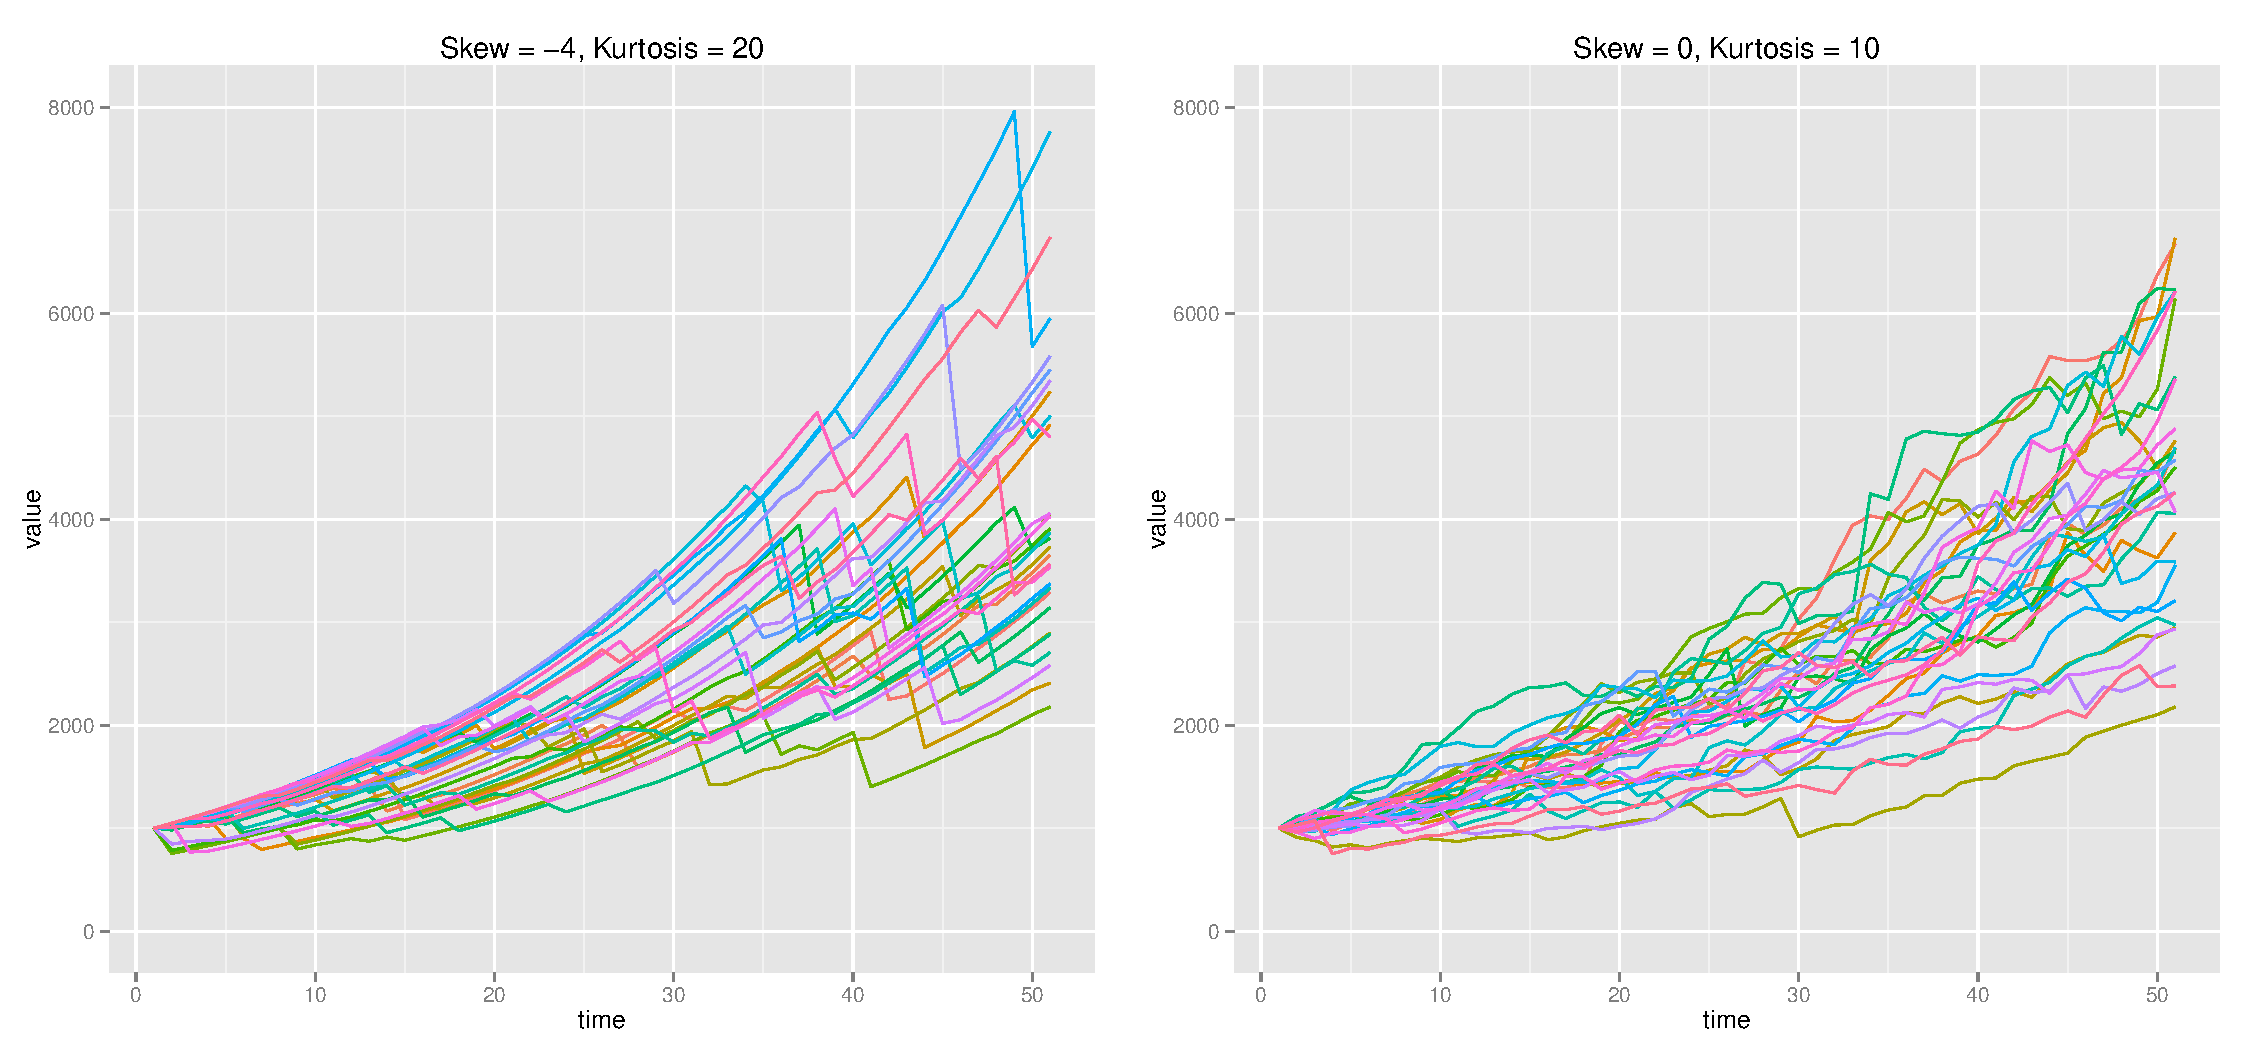
\includegraphics[width=6in]{plots/DVApaths2.pdf}
\caption{Dollar value of portfolio under different return distributions}
\label{fig:Densities}
\end{center}
\end{figure}

In Figure \ref{fig:Densities}, the simulated paths on the left and right graphs are generated from two different distributions
that have the same mean and variance, but different skewness and kurtosis. They have distinctly different return profiles.
The return paths on the left have frequent positive returns, but large losses, sometimes more than half of portfolio values.
This is not a risk a typical pensioner should take on their pension investments. However, Sharpe ratio does not distinguish
between the two portfolio return profiles. There is a necessecity for a new measure that captures the higher moments in
portfolio returns such as skewness and kurtosis.

Suppose a distribution is defined on the interval [a,b]. Let F(x) be its cumulative distribution function for the
distribution of interest. Then for any given loss threshold L, the $\Omega(\cdot)$ of the distribution is defined as:

\begin{align}
\Omega(L) = \frac{\int_L^b[1-F(r)]\mathrm{d}r}{\int_a^L F(r)\mathrm{d} r}
\end{align}

This definition makes no parametric assumption and is applicable to almost all distributions. It is also highly
intuitive because the loss threshold L can be adjusted to fit the current investment conditions. During economic
boom, L can be set to the market return to assess an investment's return against the market. During economic
downturn, L can be set to 0 to determine an investment's ability to limit loss and preserve capital.
Unlike some risk measures, such as value-at-risk,  $\Omega$ is also subadditive. In addition the $\Omega$ measure
is invariant under linear transformation of the underlying random variable X:
\begin{align}
\varphi(X) 			&= aX + b \nonumber \\
\Omega(\varphi(L)) 	&= \Omega(L) \text{ if } a > 0 \nonumber \\
\Omega(\varphi(L)) 	&= \dfrac{1}{\Omega(L)} \text{ if } a < 0
\end{align}
In order to illustrate the ability of $\Omega$ measure in capturing higher moments, we use the set of Johnson
distributions to find distributions with the same mean and variance, but different skewness and kurtosis.
The Johnson family of distributions is a set of distributions where the first four moments can be specified
given appropriate choice of parameters. The family consists of random variables z such that z becomes normal
when it is appropriately transformed.
\begin{align}
y = a + b \times g(\dfrac{z-c}{d}), \hspace{4mm} y \sim N(0,1)
\label{eq:distribution}
\end{align} 
Where $a$ and $b$ are shape parameters, $c$ is a location parameter, $d$ is a scale parameter and $g$ is one of the following four functions:
\begin{align}
g(u) = 
\begin{cases}
\ln(u) \hspace{25mm} &\text{lognormal family}\\
\ln(u + \sqrt{u^2+1}) &\text{unbounded family}\\
\ln\big(\dfrac{u}{1-u}\big) &\text{bounded family}\\
u &\text{normal family}
\end{cases}
\label{eq:Cases}
\end{align}

%%%%%%%%%%%%%%%%%%%%%%%
Given the first four moments, \cite{hill1976} discussed an algorithm for determining the associated Johnson family parameters.
Denoting $S_L$, $S_U$ and $S_B$ as the lognormal, unbounded and bounded cases of Equation (3) respectively, the algorithm is as follows:

Letting $\sqrt{\beta_1} = \dfrac{\mu_3}{\sigma^3}$, $\beta_2 = \dfrac{\mu_4}{\sigma^4}$ and $\omega = e^{-b^2}$, first solve
\begin{align}
(\omega - 1)(\omega + 2)^2 = \beta_1 \nonumber
\end{align}
Then
\begin{align}
\beta_2 &< \omega^4 + 2\omega^3 + 3\omega^2 - 3 \Longrightarrow g(\cdot) = S_B \nonumber \\
\beta_2 &> \omega^4 + 2\omega^3 + 3\omega^2 - 3 \Longrightarrow g(\cdot) = S_U \nonumber \\
\beta_2 &= \omega^4 + 2\omega^3 + 3\omega^2 - 3 \Longrightarrow g(\cdot) = S_L \nonumber
\end{align}

\underline{For $S_L$}
\begin{align}
b &= \ln(\omega)^{-{\frac{1}{2}}} &a& = \dfrac{1}{2}b\times \ln\Big(\dfrac{\omega (\omega -1)}{\sigma}\Big) \nonumber \\
c &= sign(\mu_3)\cdot\mu - e^{\frac{\frac{1}{2}b - a}{b}} &d& = sign(\mu_3) \nonumber
\end{align}

\underline{For $S_U$}\\

If $\beta_1 = 0$
\begin{align}
\omega = [(2\beta_2 - 2 )^{\frac{1}{2}} - 1]^{\frac{1}{2}}, \hspace*{5mm} b = (\ln\omega)^{-\frac{1}{2}}, \hspace*{5mm} a = 0 \nonumber
\end{align}
If $\beta_1 \neq 0$
\begin{align}
\omega_1 = [(2\beta_2 - 2.8\beta_1 - 1)^{\frac{1}{2}} - 2]^{\frac{1}{2}} \nonumber
\end{align}
as an initial estimate and $\omega$, a and b are found using the \citet{johnson1969} iterative method 

Then c and d are found using
\begin{align}
\sigma^2 &= \dfrac{1}{2}d^2(\omega - 1)(\omega cosh\Big(\dfrac{2a}{b}\Big) + 1) \nonumber \\
\mu 	 &= c - d\omega^{\frac{1}{2}}sinh\Big(\dfrac{a}{b}\Big) \nonumber
\end{align}

\underline{For $S_B$}
\vspace*{3mm}
\begin{align}
b &= \dfrac{0.626\beta_2 - 0.408}{(3 - \beta_2)^{0.479}} \hspace*{5mm} &\text{if } \beta_2 \geq 1.8 \nonumber \\
b &= 0.8(\beta_2 - 1) &\text{otherwise} \nonumber
\end{align}
Using \cite{draper1951}, $a$ is calculated. From initial estimates of $a$ and $b$ the first 6 moments are calculated using \cite{draper1952}
and then Newton-Rhapson is used to solve for $a$ and $b$, and the first two moments are then used to determine $c$ and $d$.

Then we can simulate from the Johnson random variable using
\begin{align}
z = c + d \times g^{-1}\Big(\dfrac{y - a}{b}\Big)
\end{align}
with
\begin{align}
g^{-1}(u) = 
\begin{cases}
e^u \hspace{25mm} &\text{lognormal family}\\
(e^u - e^{-u})/2 &\text{unbounded family}\\
1/(1 + e^{-u}) &\text{bounded family}\\
u &\text{normal family}
\end{cases}
\end{align}
%%%%%%%%%%%%%%%%%%%%%%%
\newpage
\section{Results and Discussion}
\subsection{Simulations}
To analyze the effects of upper moments on $\Omega$ we simulated returns from Johnson distributions with constrained mean and variance.
The empirical return distributions are shown in Figure \ref{fig:Densities}. Code for generating these figures in included in the Appendix,
which makes use of the R package contributed by \cite{mcleod2012}.

\begin{figure}[H]
\begin{center}
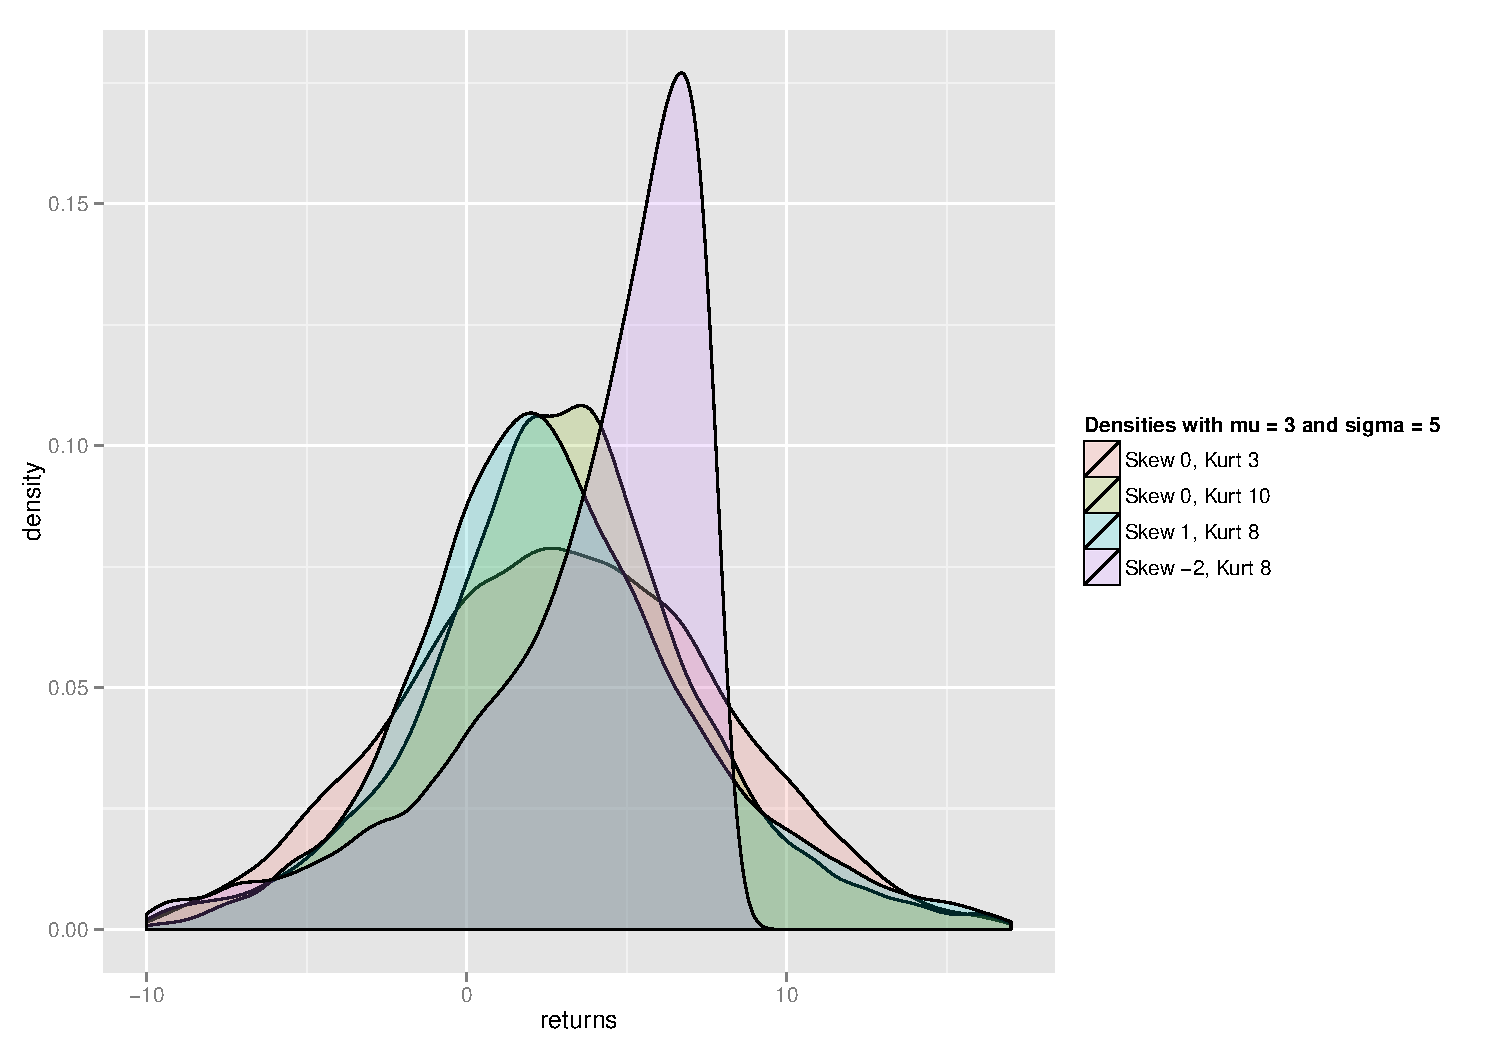
\includegraphics[width=6in]{plots/Densities.pdf}
\caption{Empirical densities for returns generated from Johnson distributions}
\label{fig:Densities}
\end{center}
\end{figure}

The $\Omega$ values for various loss levels for these return distributions are shown in Figures \ref{fig:Omegas} and \ref{fig:OmegasZoom}. 
As seen in Figure \ref{fig:Omegas}, $\Omega$ measure differentiates these four different distributions, particularly for loss threshold L
smaller than the mean $\mu$. Skewness plays a larger role in differentiating the $\Omega$ measure and higher positive skewness is preferred.
Though kurtosis' role is small compared with skewness, larger kurtosis seems to be preferred when skewness is 0 for low levels of L while less kurtosis is
preferred for higher values of L.

\begin{figure}[H]
\begin{center}
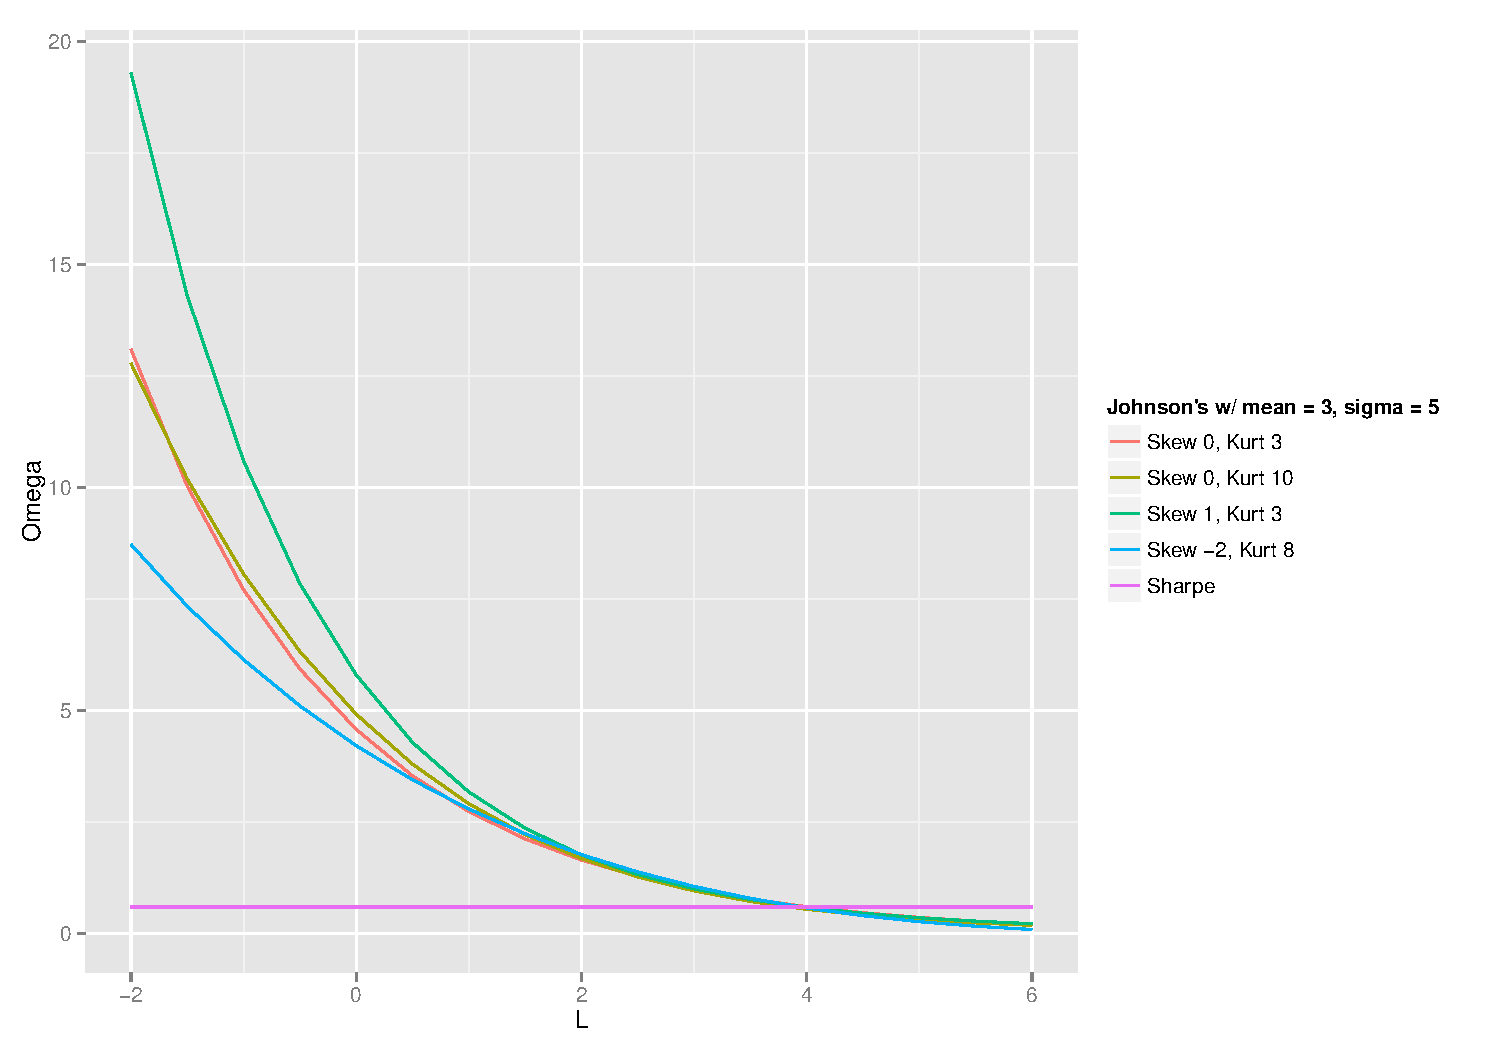
\includegraphics[width=4.5in]{plots/Preferences.pdf}
\caption{Omegas for the simulated Johnson returns}
\label{fig:Omegas}
\end{center}
\end{figure}

\begin{figure}[H]
\begin{center}
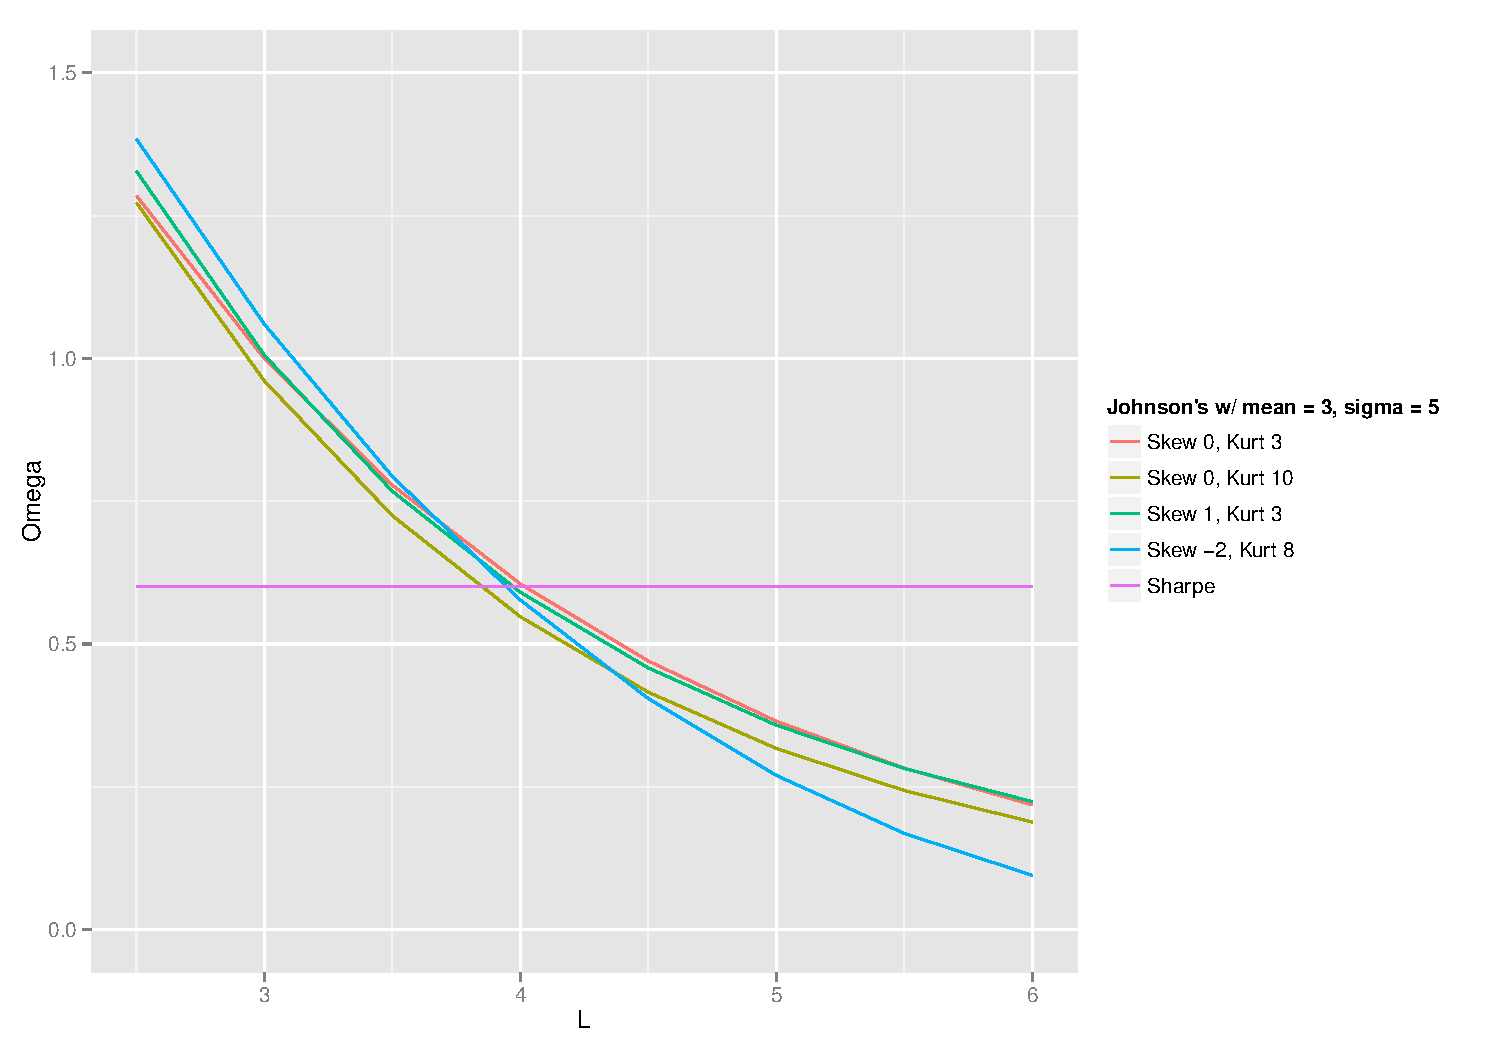
\includegraphics[width=4.5in]{plots/PreferencesZoom.pdf}
\caption{Omegas for the simulated Johnson returns}
\label{fig:OmegasZoom}
\end{center}
\end{figure}


\subsection{Empirical}

\begin{figure}[H]
\begin{center}
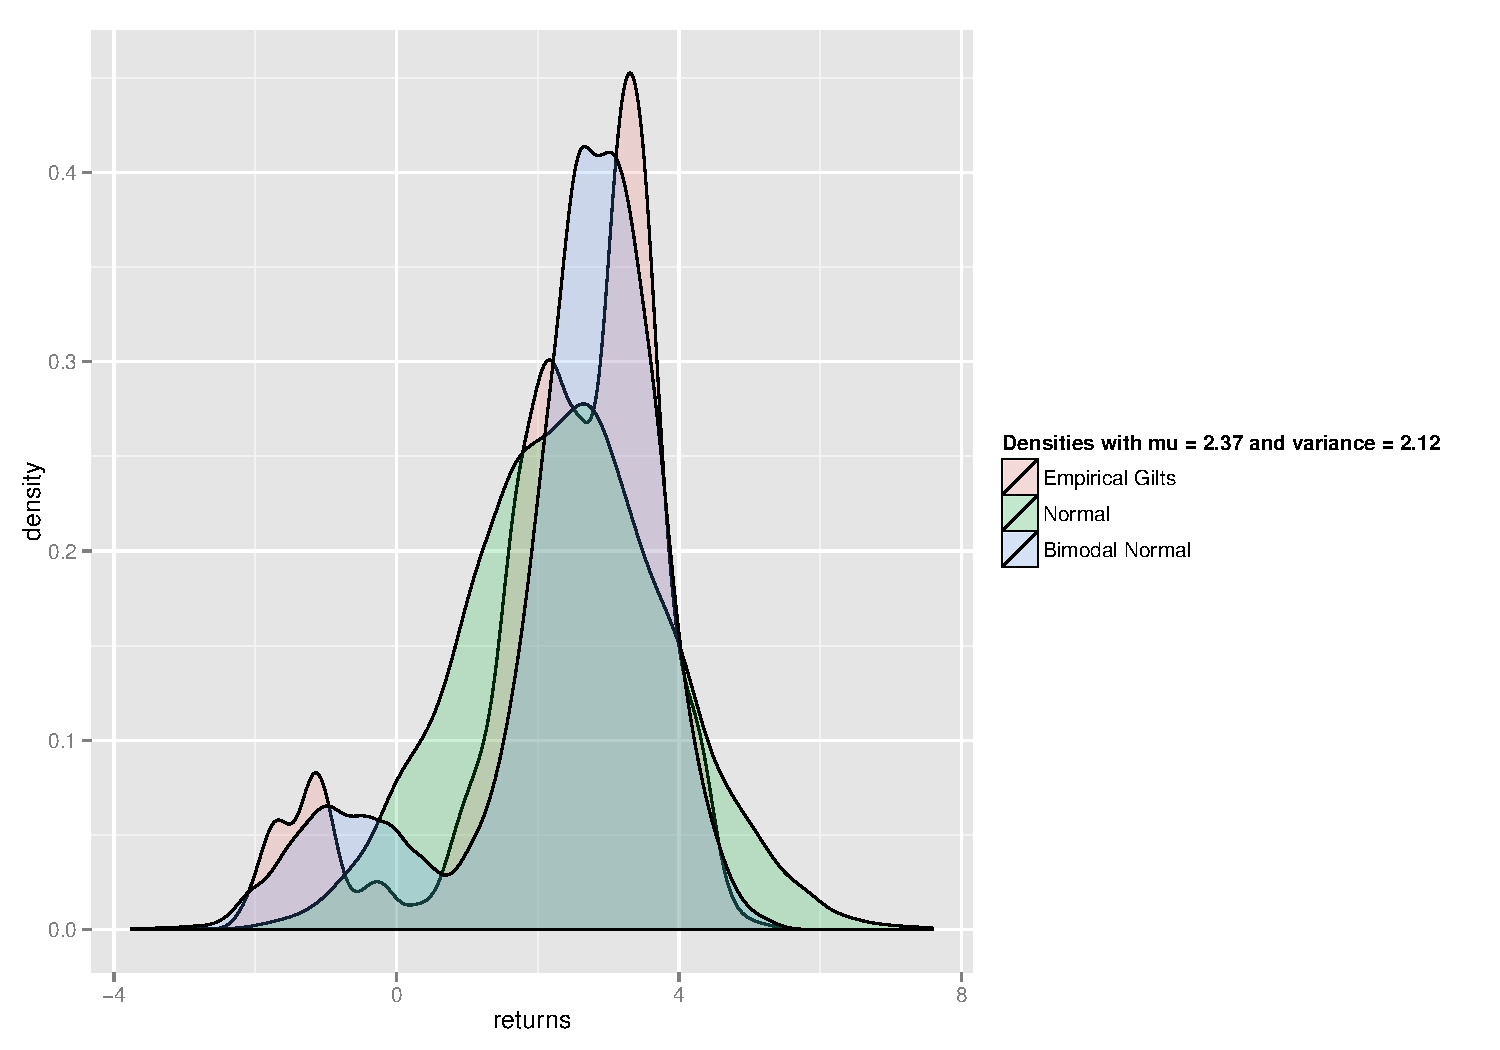
\includegraphics[width=6in]{plots/EmpiricalDensities.pdf}
\caption{Densities for empirical Gilt returns and normal and bimodal returns with equivalent first two central moments}
\label{fig:EmpiricalDensities}
\end{center}
\end{figure}

Many assets do not follow normal distributions and may possess higher moments that Sharpe ratio cannot capture.
The British treasury bonds, called gilts, are one example. We obtained 25 years of daily returns of 1-year-maturity
inflation-indexed gilts from Bank of England. The pink region in Figure \ref{fig:EmpiricalDensities} demonstrates
the empirical density. It is highly non-Gaussian and appears to have two peaks - implying a bimodal density structure.
We attempt to model this empirical distribution. A normal distribution, shown as the blue region, is first fitted.
A mixture normal distribution, which is a linear combination of two normal densities, is also fitted and shown as the
green region. By construction of fitted normal and mixture normal distributions, all three distributions have the
same mean of 2.37 and same variance of 2.12. Therefore, they cannot be distinguished by the 	Sharpe ratio.
It is apparent that the mixture normal distribution models the empirical data much better than the normal distribution.

\begin{figure}[H]
\begin{center}
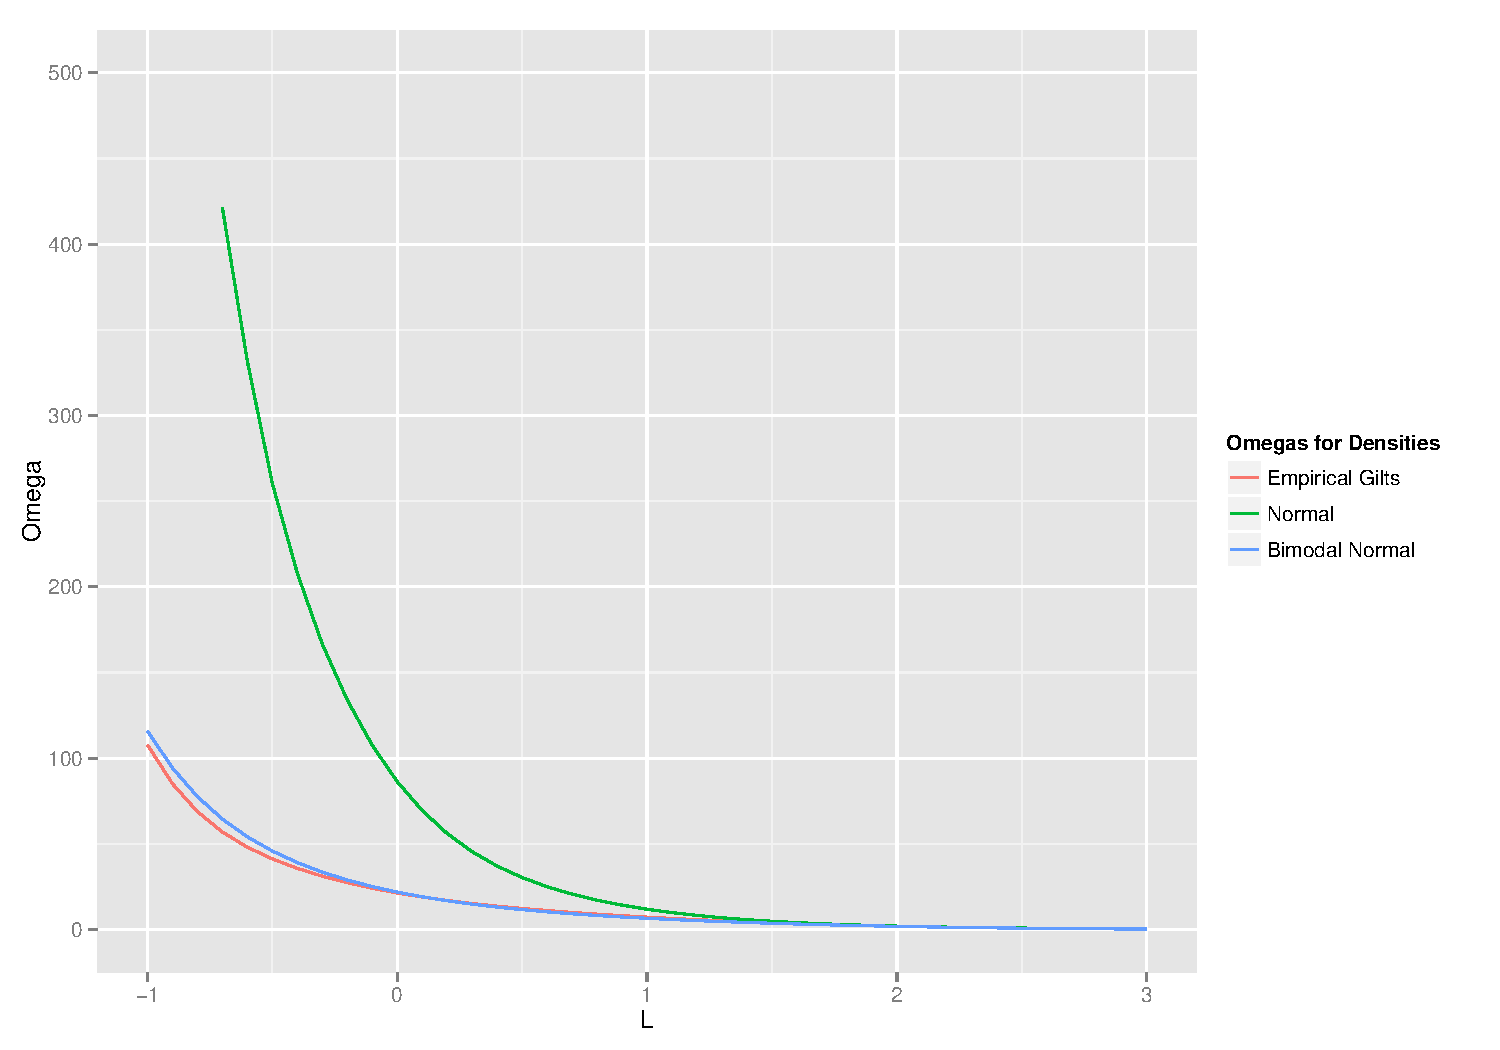
\includegraphics[width=6in]{plots/EmpiricalOmegas.pdf}
\caption{Omegas for empirical Gilt returns and normal and bimodal returns with equivalent first two central moments}
\label{fig:EmpiricalOmegas}
\end{center}
\end{figure}

The $\Omega$ measure is applied to the empirical data itself as well as simulations generated from the fitted normal
and mixture normal distributions. The results are shown in Figure \ref{fig:EmpiricalOmegas}. $\Omega$ measure is able to capture the differences
in higher moments between the three distributions. As seen in Figure \ref{fig:EmpiricalOmegas}, normal distribution fits the data poorly as
the $\Omega$ measure of the normal distribution is far from the empirical observation. Mixture normal distribution
fits the empirical data much closer. As indicated by theory, the $\Omega$ measures tend to one as the loss
threshold L tends to the mean 2.37. It is interesting to note that the mixture normal distribution is fitted to have
the same first five moments as the empirical data. The slight difference in $\Omega$ measures between the mixture
normal distribution and the empirical data indicates the $\Omega$'s ability to  detect differences in even higher
moments than the 5th moment.

\newpage
\section{Summary}
$\Omega$ measure, unlike Sharpe ratio, is designed to capture differences in higher moments between distributions.
Its capability has been shown in both simulated and empirical settings. In addition, it has some attractive features,
such as non-parametric definition and the flexibility of the loss threshold. Non-parametric definition removes
estimation errors and allows quick estimation of the $\Omega$ measure even for complex portfolios - using the
empirical quantiles as the CDF. Flexibility of the loss threshold allows the investor to choose a threshold that
best fits the investor's risk apetite.

The $\Omega$ measure is not without drawbacks. It is possibly unbounded for a distribution defined on an infinite interval.
It carries similar estimation issues as other risk measures that focus on the tail. This means $\Omega$ measure does
not make sense unless we observe sufficient amount data below or ablove the risk threshold L. In addition, when the
L is set to the mean of the distribution, i.e. L = $\mu$, $\Omega$ is equal to 1 and therefore does not distinguish
any distributions with the same mean.

Despite its drawbacks, $\Omega$ measure still provides a useful alternative to the Sharpe ratio, particularly for
complex and non-Gaussian portfolios. This measure extends naturally to hedge funds, who by nature take large bets in
unconventional and complex strategies. It would be of particular interest to look at how rankings of hedge fund
returns would change using the $\Omega$ measure instead of the Sharpe ratio. It is also clear that the $\Omega$ measure
becomes more stable as more empirical data becomes available. It is thus interesting to examine its convergence rate
with respect to the amount of data. In addition, volatility estimates are known to become more accurate when the
sampling frequency is increased. Whether $\Omega$ measure has this property remains to be tested.
These areas pave a way to new areas of research into the $\Omega$ measure and further tests its applicability in practice.

%%%%%%%%%%%%%%%%%%%% BACKMATTER %%%%%%%%%%%%%%%%%%%%%%%%%%%%

\newpage
\addcontentsline{toc}{section}{References}
\bibliography{906References}

\newpage
\begin{appendices}
%\renewcommand{\thesection}{A.\arabic{section}}
\renewcommand\thefigure{\thesection.\arabic{figure}}
%\gdef\thesection{Appendix \Alph{section}}
\section{}
\setcounter{figure}{0}

\lstinputlisting{Omega.r}
\lstinputlisting{JohnsonGenerate.r}
\lstinputlisting{DistributionComparison.r}

\end{appendices}

\end{document}
